\section{The Advantage and Challenge of Vector Boson Fusion}
\frame {
    \frametitle{Vector Boson Fusion (VBF)}

    \begin{columns}
        \begin{column}{0.4\textwidth}
            %{ \scriptsize VBF is the second highest Higgs production mechanism, but possesses a much better handle to identify the jets with than the leading mechanism, gluon-gluon fusion. }

            \begin{figure}
                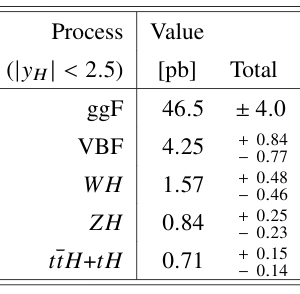
\includegraphics[width=\linewidth,height=0.5\textheight,keepaspectratio]{higgs_production_modes.png}
                \caption{\scriptsize source - arXiv:1909.02845 [hep-ex] }
            \end{figure}
        \end{column}
        \begin{column}{0.6\textwidth}
            {\scriptsize
                VBF events can be identified based on the two hight-$p_T$, large $\Delta \eta$ jets (called  {\it signature jets})
            }
            \begin{center}\resizebox{0.40\textheight}{!}{ \begin{tikzpicture} \begin{feynman}
    \vertex (a);
    \vertex [right=of a] (b) {H};
    \vertex [above left=of a] (vb1);
    \vertex [below left=of a] (vb2);
    \vertex [left=of vb1] (q1i) {q};
    \vertex [left=of vb2] (q2i) {q};
    \vertex [above =of b] (q1f) {q};
    \vertex [below =of b] (q2f) {q};

    \diagram* {
        (q1i) -- (vb1) -- (q1f),
        (q2i) -- (vb2) -- (q2f), 
        (vb1) -- [boson] (a) -- [boson] (vb2),
        (a) -- [scalar] (b),
    };
\end{feynman} \end{tikzpicture}
 }\end{center}

            {\scriptsize
                At leading order, ggF results in only the decay products of the Higgs itself
            }
            \begin{center}\resizebox{0.40\textheight}{!}{ \begin{tikzpicture} \begin{feynman}
    \vertex (c);
    \vertex [above left=of c] (a);
    \vertex [below left=of c] (b);
    \vertex [left=of a] (gluon1) {g};
    \vertex [left=of b] (gluon2) {g};
    \vertex [right=of c] (higgs) {H};

    \diagram* {
        (gluon1) --[gluon] (a),
        (gluon2) --[gluon] (b),
        (c) --[scalar] (higgs),
        (a) -- (b) -- (c) -- (a)
    };
\end{feynman} \end{tikzpicture}
 }\end{center}
        \end{column}
    \end{columns}
}

\frame {
    \frametitle{ My Goal: Increase Discrimination Between VBF and ggF }

    \begin{columns}
        \begin{column}{0.4\textwidth}
            ggF events can produce radiation than makes them look like VBF events.
            Events must be properly tagged to avoid diluting statistics.
        \end{column}
        \begin{column}{0.6\textwidth}
            \begin{center}\resizebox{0.40\textheight}{!}{ \begin{tikzpicture} \begin{feynman}
    \vertex (a);
    \vertex [right=of a] (b) {H};
    \vertex [above left=of a] (vb1);
    \vertex [below left=of a] (vb2);
    \vertex [left=of vb1] (q1i) {q};
    \vertex [left=of vb2] (q2i) {q};
    \vertex [above =of b] (q1f) {q};
    \vertex [below =of b] (q2f) {q};

    \diagram* {
        (q1i) -- (vb1) -- (q1f),
        (q2i) -- (vb2) -- (q2f), 
        (vb1) -- [boson] (a) -- [boson] (vb2),
        (a) -- [scalar] (b),
    };
\end{feynman} \end{tikzpicture}
 }\end{center}
            \begin{center}\resizebox{0.40\textheight}{!}{ \begin{tikzpicture} \begin{feynman}
    \vertex (c);
    \vertex [above left=of c] (a);
    \vertex [below left=of c] (b);
    \vertex [left=of a] (gluon1) {g};
    \vertex [left=of b] (gluon2) {g};
    \vertex [right=of c] (higgs) {H};

    \diagram* {
        (gluon1) --[gluon] (a) 
        (gluon2) --[gluon] (b)
        (c) --[scalar] (higgs)
        (a) -- (b) -- (c) -- (a)
    };
\end{feynman} \end{tikzpicture}
 }\end{center}
        \end{column}
    \end{columns}
}
